\clearpage
\section{Externality (definice, kladné externality, záporné externality, řešení externalit).}
\subsection{Definice}
\begin{itemize}
    \item Efekt přelévání
    \item Nastává, pokud výroba/spotřeba subjektu způsobuje nezamýšlené náklady nebo přínosy jiným subjektům, 
    aniž by ti, kteří tyto náklady nebo příjmy způsobují, za ně platili
    \item Podstata je porušení něčího práva
    \item Vyvolávají neefektivnost, vedou k neoptimálnímu objemu výroby, neefektivní alokace zdrojů
    \item Není nedokonalost trhu, ale situace, kdy tržní vztahy teprve vznikají
    \item Ve výrobě i v spotřebě
    \item Vztah, který není postižen systémem cen
\end{itemize}

\subsection{Záporné externality}
\begin{itemize}
    \item Někdo na někoho přenese náklady a on s tím nesouhlasí
    \item Nesoulad mezi soukromými a společenskými náklady (společenské n. jsou veškeré n. vyvolané výrobou statku)
    \item Výrobci vyrábějí více, než by vyráběli, kdyby museli nést veškeré společenské náklady
    \item \textbf{Soukromě optimální množství statku je větší než společensky optimální množství.}
    \item Příklad:
    \begin{itemize}
        \item Uhelná elektrárna poškozuje lesy v okolí, majitelé lesa mají škody, elektrárna je nemusí platit.
        \item $MC_P$ jsou mezní náklady elektrárny, $MC_S$ jsou společenské náklady, $D$ je poptávka, nabídka
        je totožná s $MC_P$
        \item Vyrábět se bude množství $Q_P$, ale společensky optimální by bylo množství $Q_S$
        
        
        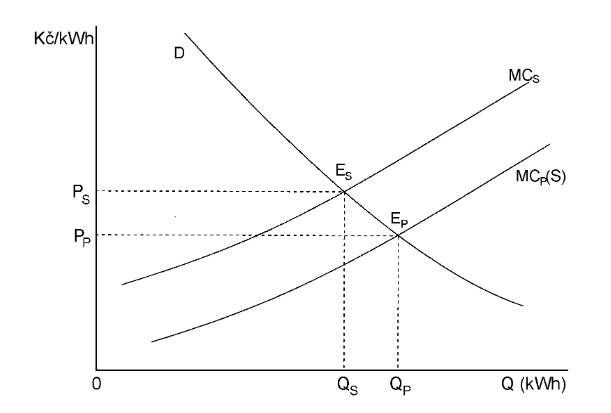
\includegraphics[width=15cm]{images/22_zaporne.png}
    \end{itemize}
\end{itemize}

\subsection{Kladné externality}
\begin{itemize}
    \item Činnost jednoho ekonomického subjektu přináší prospěch jinému, přičemž jej tento nemusí hradit
    \item Příklad:
    \begin{itemize}
        \item Majitelé lesa způsobují prospěch v obcích v okolí, lidé jim za to nic neplatí
        \item Majitelé lesa budou chtít udržovat menší plochu lesa, než by bylo společensky optimální množství
        
        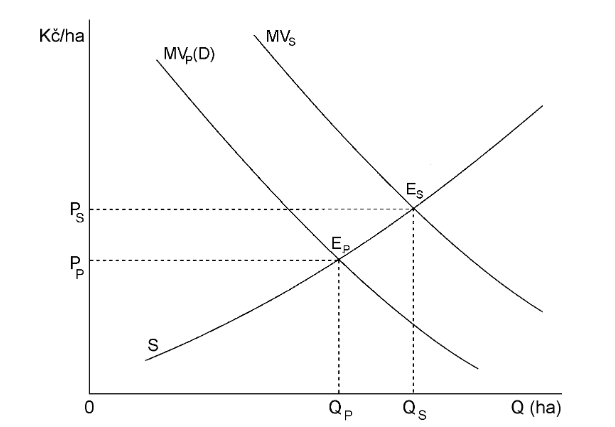
\includegraphics[width=15cm]{images/22_kladne.png}
    \end{itemize}
\end{itemize}

\subsection{Řešení externalit}
\begin{itemize}
    \item Zásahy státu - dotace subjektům s pozitivní externalitou, daně/kvóty subjektům se zápornou externalitou
    \item Soukromým vyjednáváním (pokud nejsou vysoké náklady na nalezení subjektů k vyjednávání a na dodržování
    dohod - \uv{transakční náklady})
    \item Je o domluvě, která strana ponese dodatečné náklady
    \item U záporných externalit většinou neexistuje nulová škoda, ale optimální škoda (příklad: prach v domě, nikdo
    nemá 0 prachových částic v domě)
    \item U záporných externalit je vhodné propojení s legislativou, aby dodatečné břemeno leželo na straně škůdce a ne
    poškozovaného
    \item Častá překážka - vysoké transakční náklady (vyhledání škůdce, prokázáni viny, vedení soudního řízení ->
    obětované příležitosti), řešením jsou právě státní zásahy, ale až v druhé řadě
    \item Coaseho teorém - pokud nebrání dohodě dodatečné náklady, lidé dosahují efektivních řešení domluvou
    \item Piguova daň - zdaňuje negativní externalitu, dotuje pozitivní externalitu
\end{itemize}